\documentclass[handout, 10pt]{beamer}
\usepackage[hangul]{kotex}
\usepackage[T1]{fontenc}

% other packages
\usepackage{natbib}
\usepackage{graphicx,float,pstricks,listings,stackengine,xcolor,calligra}
\usepackage{amsmath,amssymb,latexsym}
\usepackage{booktabs,longtable,multicol,multirow,lscape,rotating}
\usepackage{caption,subcaption}
    \newcommand{\source}[1]{\subcaption*{\raggedright 자료: {#1} } }
\usepackage{threeparttable} % Align column caption, table, and notes
%\usepackage{adjustbox} % Shrink stuff
%\usepackage{showframe} % Useful for debugging

\author{오성재}
\title{박사학위 논문개요}
%\subtitle{}
\institute{서울대학교 경제학과 박사과정 \\ 박사학위 논문심사}
\date{\today}
\usetheme{Darmstadt}
%\usepackage{warehouse/PekingU}

% defs
\def\cmd#1{\texttt{\color{red}\footnotesize $\backslash$#1}}
\def\env#1{\texttt{\color{blue}\footnotesize #1}}
\definecolor{deepblue}{rgb}{0,0,0.5}
\definecolor{deepred}{rgb}{0.6,0,0}
\definecolor{deepgreen}{rgb}{0,0.5,0}
\definecolor{halfgray}{gray}{0.55}

\lstset{
    basicstyle=\ttfamily\small,
    keywordstyle=\bfseries\color{deepblue},
    emphstyle=\ttfamily\color{deepred},    % Custom highlighting style
    stringstyle=\color{deepgreen},
    numbers=left,
    numberstyle=\small\color{halfgray},
    rulesepcolor=\color{red!20!green!20!blue!20},
    frame=shadowbox,
}


\begin{document}

\begin{frame}
    \titlepage
    %\begin{figure}[htpb]
        %\begin{center}
            %
\includegraphics[width=0.2\linewidth]{pic/PKU_logo.png}
        %\end{center}
    %\end{figure}
\end{frame}

%\AtBeginSection[]
%{
  %\begin{frame}
    %\frametitle{Table of Contents}
    %\tableofcontents[sectionstyle=show,subsectionstyle=show/shaded/hide,subsubsectionstyle=show/shaded/hide,currentsection]
  %\end{frame}
%}

\begin{frame}
    \frametitle{Table of Contents}
    \tableofcontents[sectionstyle=show,subsectionstyle=show/shaded/hide,subsubsectionstyle=show/shaded/hide]
\end{frame}

\section{들어가는 글}
\begin{frame}{들어가는 글}
    \begin{itemize}
        \item 기회불평등 개념 소개
        \item 연구방법 소개
        \begin{itemize}
            \item 각종 기회불평등 지수 : 지니기회불평등지수, 개천용기회불평등지수, Theil-0응용 지수 등등.
            \item 1차(2차) 확률지배 개념 및 검증법.
            \item 주성분분석(PCA)을 활용한 환경 구분.
        \end{itemize}
        \item 이하 각 장은 선행연구 소개, 자료소개 및 연구결과로 구성.
    \end{itemize}
\end{frame}

\section{기회불평등과 경제성장}
\begin{frame}{기회불평등과 경제성장}
    \begin{itemize}
        \item 불평등이 경제성장에 미치는 영향을 연구한다.
        \item PISA와 TIMSS라는 두 국제교육평가 자료를 이용하여 교육의 불평등을 측정하고 이를 기회불평등과 노력불평등으로 분해한다.
        \item 교육불평등과 노력불평등이 경제성장룰에 미치는 영향을 성장회귀 분석을 통해 살펴본다.
    \end{itemize}
\end{frame}

\section{대학수학능력시험을 통해 살펴본 교육성취의 기회불평등}
\begin{frame}{대학수학능력시험을 통해 살펴본 교육성취의 기회불평등}
    \begin{itemize}
        \item 수학능력시험 성적을 이용하여 부모의 학력 또는 부모의 소득수준이 학생의 성적에 얼만큼 영향을 주는지 한국의 자료를 이용하여 연구한다.
        \item 한국교육고용패널(KEEP)의 2005학년도 수능성적과 한국교육종단연구(KELS)의 2011학년도 수능성적을 활용한다.
        \item 연구결과 언어, 외국어 두 영역 모두 기회불평등이 존재했다. 외국어 영역에서 기회불평등의 정도가 더 심각 했다. 환경적으로는 남성보호자의 학력을 환경으로 했을때의 기회불평등 정도가 가구소득의 경우보다 더 높게 나타났다. 지역적으로는 농$/cdot$어촌 출신 학생이 이외의 학생에 대하여 기회불평등한 상황이므로 이들에 대한 지역균형선발과 같은 정책이 의미 있음을 확인했다.
    \end{itemize}
\end{frame}

\section{대학입학과 청년의 경제적 성취의 기회불평등}
\begin{frame}{대학입학과 청년의 경제적 성취의 기회불평등}
    \begin{itemize}
        \item 한국에서 좋은 대학에 들어가는데 있어 환경의 영향력이 얼마인지 그 추이를 살펴본다.
        \item 또한 이들이 사회 초년생으로 얻는 첫 임금과 같은 대학의 QS순위 및 대학졸업 후 2년안에 획득한 월급을 성취로 한다.
        \item 대학진학의 경우 조사년도 전반에 걸쳐 기회불평등이 존재하는 것으로 나타났다. 2007년을 절정으로 이전에는 기회불평등이 상승세였다가 줄어드는 모습으로 보인다. 가장 열악한 환경에 놓인 학생이 최상위권 대학의 진학에 실패할 확률은 70\%에 달해 해당 대학들의 현재 기회균등 전형이 더욱 확대되어야 할 필요가 있다. 2007년 이후 기회불평등의 감소추세와 정시, 수시간의 선발비율 변화의 관련성에 대한 추가 연구가 필요하다.
    \end{itemize}
\end{frame}

\section{한국의 경제적 기회불평등}
\begin{frame}{한국의 경제적 기회불평등}
    \begin{itemize}
        \item 한국의 가계소득 획득에서 기회불평등 추이를 살펴본다.
        \item 한국노동패널(KLIPS)의 1차-22차 자료를 활용한다.
    \end{itemize}
\end{frame}

\begin{frame}
  \begin{figure}[htpb]
        \begin{center}
            \caption{가구주부친 학력환경하 가구소득의 기회불평등 추이}
            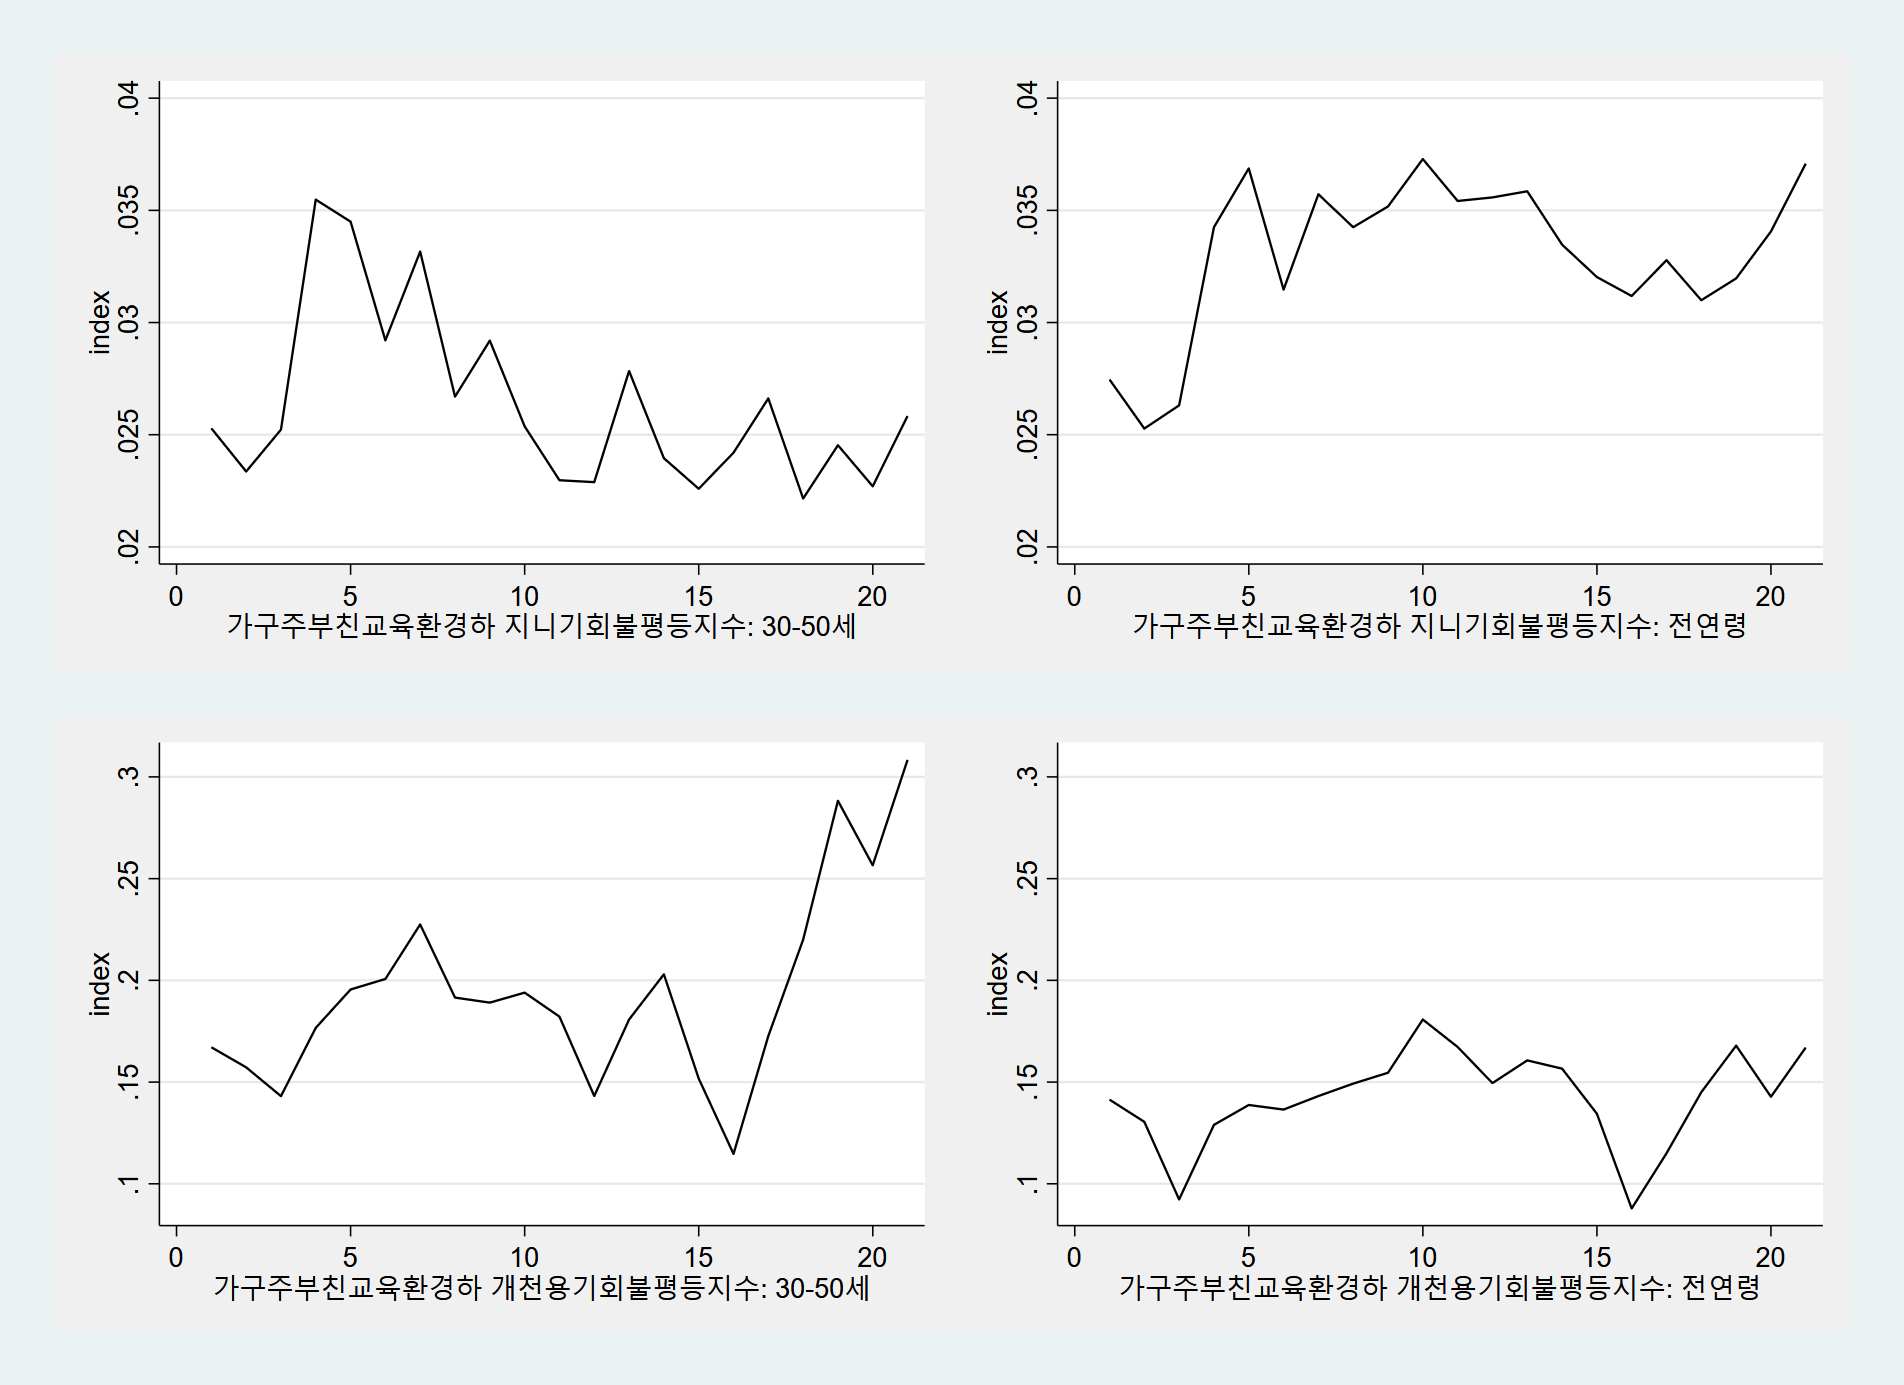
\includegraphics[scale=0.15]{incn1tm_edugrp.png}
        \end{center}
    \end{figure}
\end{frame}

\begin{frame}
  \begin{figure}[htpb]
        \begin{center}
            \caption{가구주부친 직업환경하 가구소득의 기회불평등 추이}
            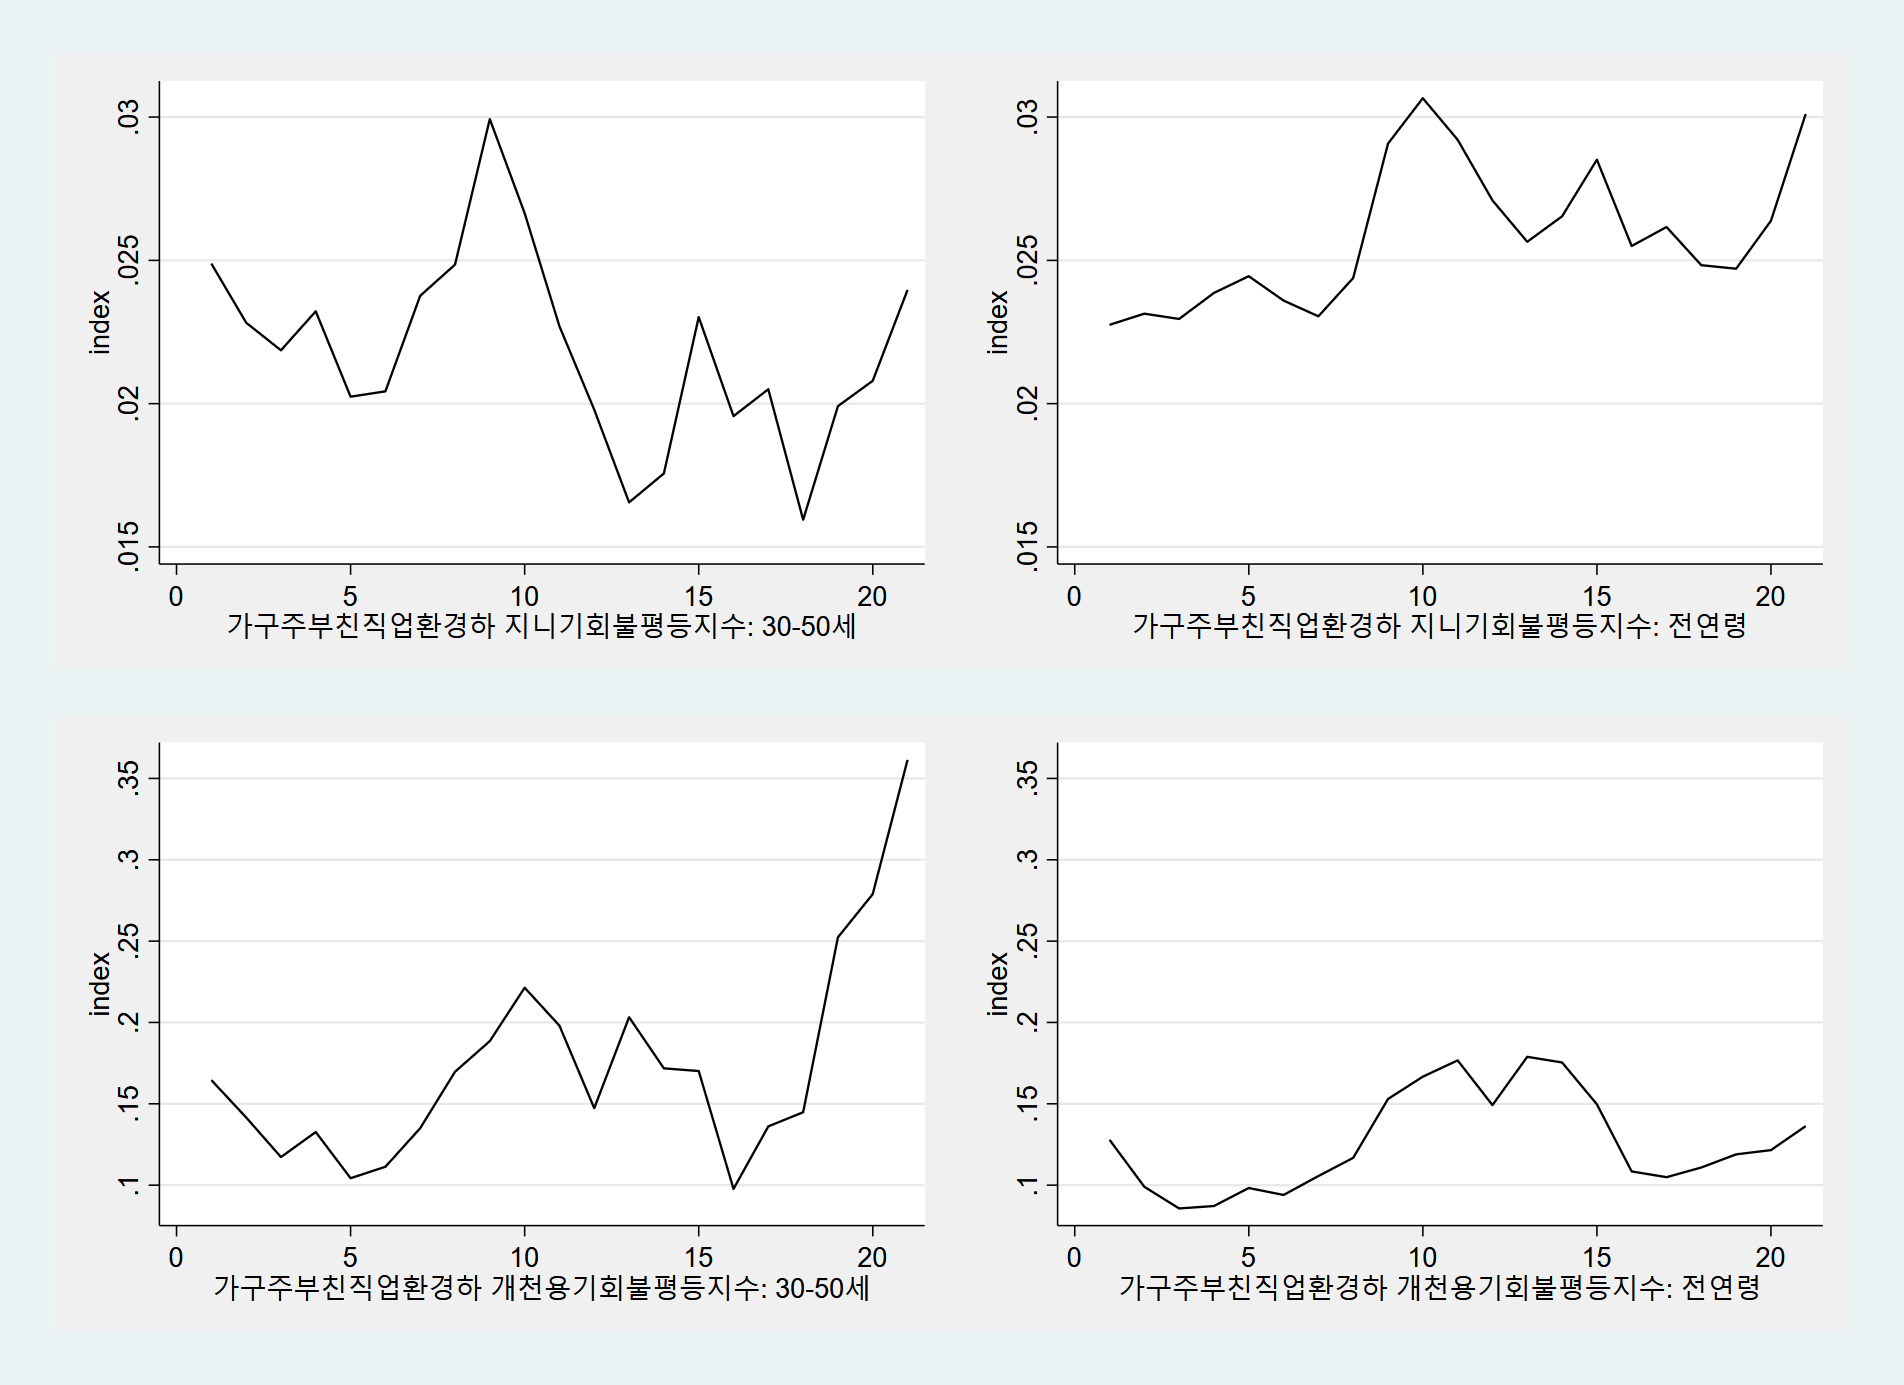
\includegraphics[scale=0.15]{incn1tm_jobgrp.png}
        \end{center}
    \end{figure}
\end{frame}

\section{맺음말}
\begin{frame}{맺음말}
    \begin{itemize}
        \item 대중들이 관심을 가지는 불평등과 공정의 문제는 기회불평등을 살펴볼때 비로소 실체를 파악할 수 있다.
        \item 이를 위해, 교육성취에서 가구소득 수준까지 한국사회 전반의 기회불평등 상태를 조사하였다.
        \item 교육과정 및 복지정책에서 기회불평등 개념을 적극 도입하기를 희망한다.
    \end{itemize}
\end{frame}

\end{document}